% Couverture Thèse TPT Latex v2
% Fabrice Linot 04/12/11

\documentclass[12pt,a4paper,english]{MastersDoctoralThesis}
%\usepackage[left=2.9cm,top=0cm,right=2.6cm,bottom=1.2cm]{geometry}
\usepackage{graphicx}
\usepackage{eso-pic}
\usepackage{array}
%\usepackage[french]{babel}
\usepackage{textcomp}
\usepackage{setspace}
\usepackage{helvet}	% or \usepackage{lmodern}
\renewcommand\textnumero{n$^{\textsf{{\tiny O}}}$}
\renewcommand{\familydefault}{\sfdefault}

%----

\usepackage[utf8]{inputenc} % Required for inputting international characters
\usepackage[T1]{fontenc} % Output font encoding for international characters

\usepackage[autostyle=true]{csquotes} % Required to generate language-dependent quotes in the bibliography

\usepackage[export]{adjustbox}

% \usepackage{cite}
\def\RR{\mathbb{R}}
\usepackage{amssymb}
\usepackage[cmex10]{amsmath}
\usepackage{algorithm}
\usepackage{algorithmic}

\newtheorem{lemma}{Lemma}
\newcommand{\prox}{\mathrm{prox}}
\DeclareMathOperator*{\argmin}{arg\,min}
%----


\usepackage{ifpdf}
\newcommand\BackgroundPic{
\ifpdf
	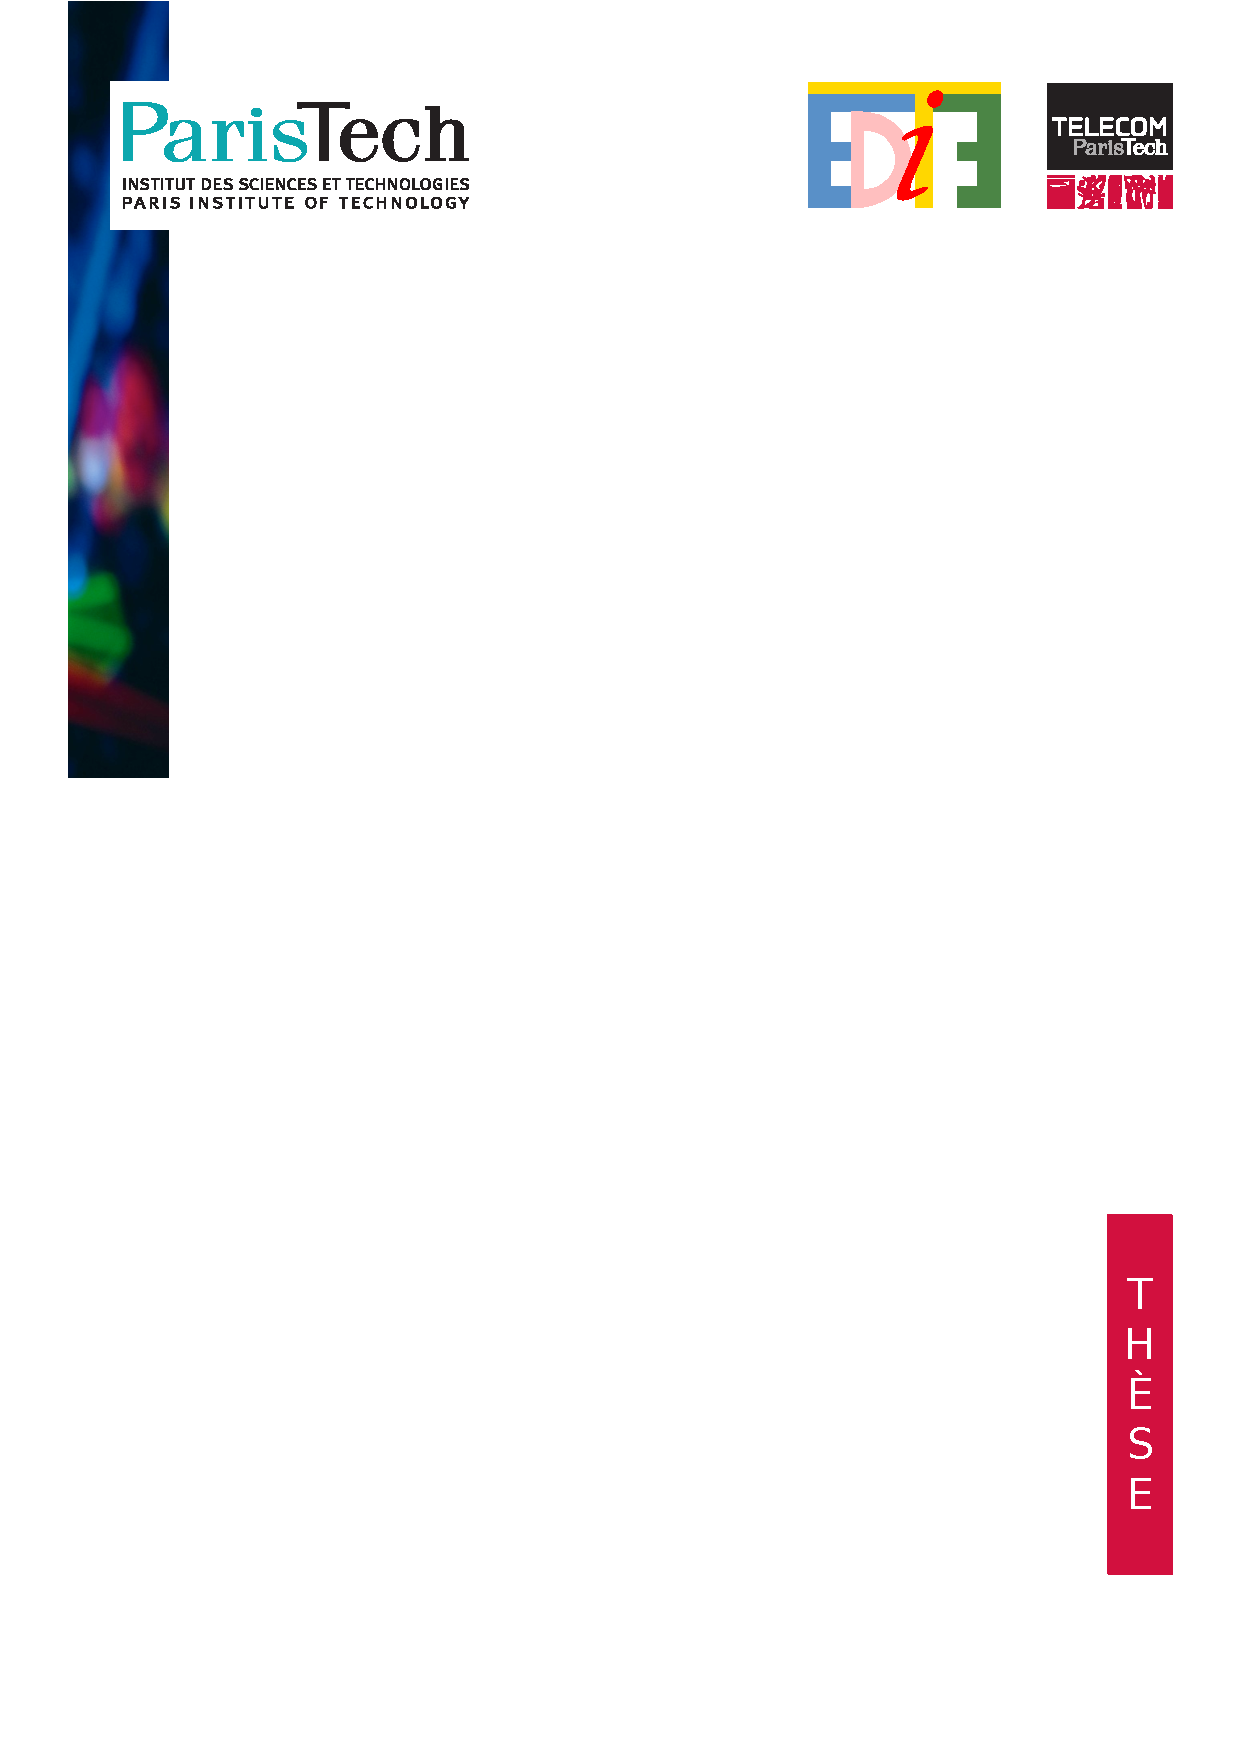
\includegraphics[height=\paperheight,width=\paperwidth]{cover_bg.pdf}
\else
	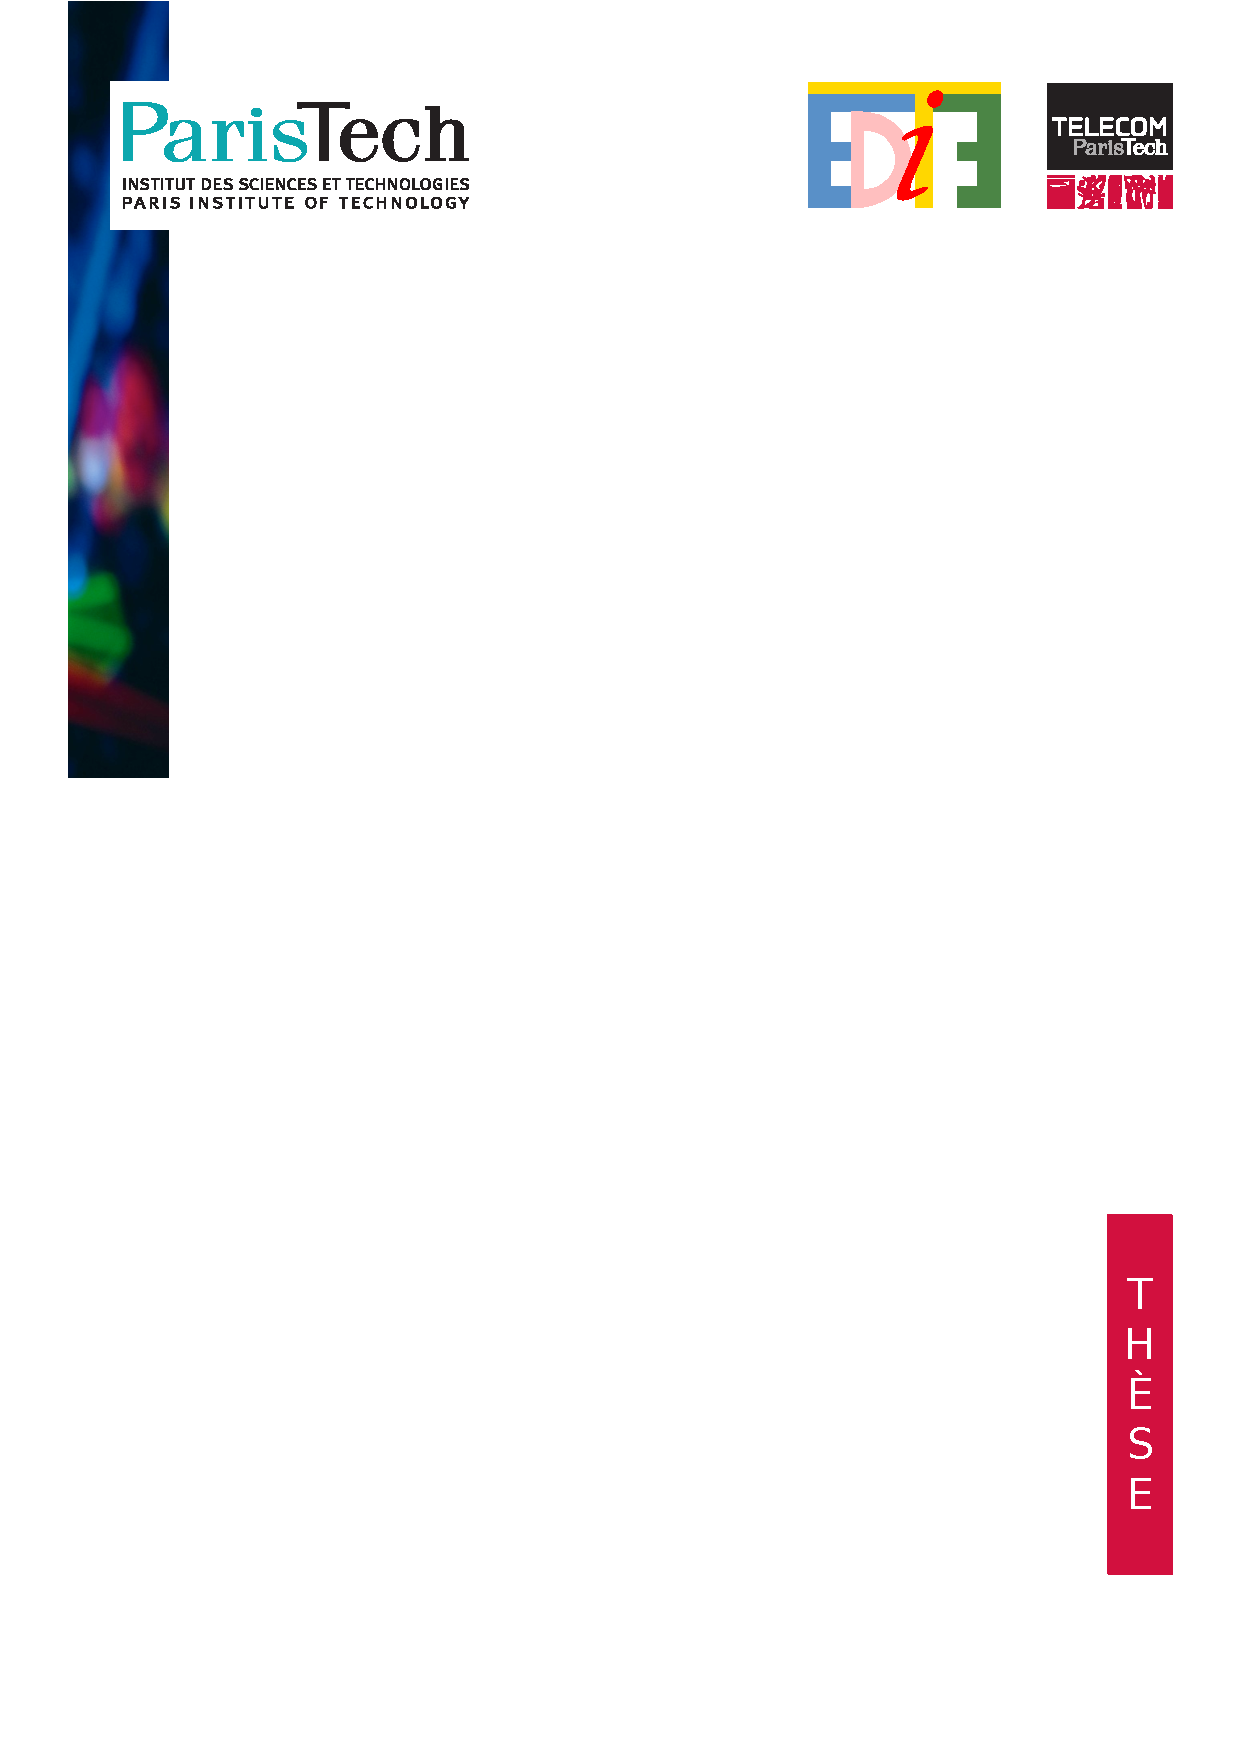
\includegraphics[height=\paperheight,width=\paperwidth]{cover_bg.pdf}
\fi}

\pagestyle{empty}

\begin{document}
\AddToShipoutPicture*{\BackgroundPic}
~
\begin{minipage}{1.05\textwidth}
\begin{flushright}
% 
\includegraphics[scale=0.45]{logo_TPT.pdf}
    \vspace{3.65cm}
    {\small {EDITE - ED130~~~~~~~2018-ENST}}
\end{flushright}
\end{minipage}


\vspace{0.0cm}
\begin{center}
%


% { {École doctorale n°130 : EDITE - Informatique, Télécommunications et Électronique}}


%
\vspace{.5cm}
%
%
%
%{\Large École doctorale \textnumero XX: texte}\\		% version une ligne
%{\Large École doctorale \textnumero XX:\\ texte}\\		% version deux lignes (changer les espaces en conséquence
%
%
%
\vspace{0.3cm}
%
%
%
{\LARGE {PhD THESIS}}\\
\vspace{0.3cm}
%{\LARGE {\bf T\hspace{0.1cm}H\hspace{0.1cm}È\hspace{0.1cm}S\hspace{0.1cm}E}}\\
{\LARGE {T\'el\'ecom ParisTech}}\\
%
%
%
\vspace{1.0cm}
%
%
%
%
{\normalsize {A dissertation submitted in partial fulfillment\\
of the requirements for the degree of}}\\
\vspace{0.3cm}
{\LARGE {\bf DOCTOR OF SCIENCE}}\\
\vspace{0.3cm}
{\Large {\bf Specialized in Signal and Image Processing}}\\
%
%
%
\vspace{1.5cm}
%
%
%
%{\normalsize {Présentée et soutenue publiquement par}}\\
\vspace{0.3cm}
{\LARGE {\bf Yousra Bekhti}}\\
\vspace{0.3cm}
{\normalsize Février 2018}\\
%
%
%
% \vfill
\vspace{1.cm}%
%
%
%
% \flushleft
% \hspace{-2.0cm}
\begin{spacing}{3.0}
\textcolor[RGB]{191,18,56}{
\noindent
{\Huge{\bf Sparse source localization for MEG/EEG brain imaging}}\\
}
\end{spacing}
%
%
\vspace{2.cm}%
% \vfill~%\vfill
%
%
%
% {\normalsize
% \begin{tabular}{c}
%     Sous la direction de : {\textbf{Andrés ALMANSA} et \textbf{ Tamy BOUBEKEUR}}
% Directeur de thèse:					{\bf Prénom NOM}\\
% Co-encadrement de la thèse:		{\bf Prénom NOM}
% \end{tabular}
% }
\end{center}
%
%
%
% \vfill
\vspace{-1.2cm}
%
%
%
\flushleft
\hspace{-1.7cm}
\begin{minipage}{1.05\textwidth}	% ou .91\textwidth si vous n'avez pas assez de place
{\bf Jury :}\vspace{0.2cm}\\
% Mme/M. Prénom NOM, Titre, Unité de recherche, Ecole
{\bf M. Thomas Rodet}, {\small Prof. ENS Paris-Saclay}
\hfill President\vspace{0.2cm}\\
{\bf Mme. Maureen Clerc}, {\small Dr. INRIA Sophia-Antipolis}
\hfill Examiner\\
{\bf M. Erki Somersalo}, {\small Prof. Case Western Reserve Univ.}
\hfill Examiner\\%\vspace{0.2cm}
{\bf M. Laurent Albera}, {\small MdC HdR Univ. Rennes}
\hfill Examiner\\
{\bf M. XXX}, {\small XXX}
\hfill Examiner\vspace{0.2cm}\\
{\bf M. Roland Badeau}, {\small T\'el\'ecom ParisTech, Paris, France}
\hfill Director\\
{\bf M. Alexandre Gramfort}, {\small T\'el\'ecom ParisTech, Paris, France}
\hfill Advisor\\
\end{minipage}\\
%
%
%
\vspace{.8cm}
%
%
%
\centering
{\bf TELECOM ParisTech}\\
{\small École de l'Institut Mines-Télécom - Membre de ParisTech}\\
{\tiny 46 rue Barrault 75013 Paris - (+33) 1 45 81 77 77 - www.telecom-paristech.fr}
%
%
%
\newpage

\end{document}
